\documentclass{article}

% NeurIPS 2024 style
\usepackage[final,nonatbib]{neurips_2024}

\usepackage[utf8]{inputenc}
\usepackage[T1]{fontenc}
\usepackage{hyperref}
\usepackage{url}
\usepackage{booktabs}
\usepackage{amsfonts}
\usepackage{nicefrac}
\usepackage{microtype}
\usepackage{graphicx}
\usepackage{subcaption}

\title{Embodied Robotic Agent for Stylistic Go Imitation}

\author{
  Ran Qi \\
  Division of Engineering Science\\
  University of Toronto\\
}

\begin{document}

\maketitle

\begin{center}
\url{https://github.com/fastwalker1118/go}
\end{center}

\begin{abstract}
Played by 40 million people worldwide, Go is an ancient strategy game where AlphaGo's 2016 victory marked the dawn of the deep reinforcement learning era. While AI engines now far surpass human professionals, their alien playing style limits adoption as practice partners. We present an embodied robotic agent that imitates the idiosyncratic playstyle of a specific human player. Our system combines three components: (1)~era-aware supervised fine-tuning of KataGo's human SL model (b18c384nbt-humanv0, ${\sim}$29M parameters) on 146,911 deduplicated professional games organized by decade, improving move prediction by up to +7.3\% absolute top-1 on era-specific held-out sets, and achieving 59.4\% top-1 accuracy on Nie Weiping's games (+7.7\% over the self-play baseline); (2)~zero-shot board perception using Grounded-SAM-2 for stone detection without task-specific training data; and (3)~a PPO-trained pick-and-place policy in NVIDIA Isaac Lab for a Franka Panda arm with a suction cup end-effector, achieving 4.2\,mm median placement error at 100\% task completion using delta-from-current actions and an online IK teacher for imitation-guided training.
\end{abstract}

%----------------------------------------------------------------------
\section{Introduction}
%----------------------------------------------------------------------

\begin{figure}[h]
\centering
\includegraphics[width=\textwidth]{Gemini_Generated_Image_uhkdpiuhkdpiuhkd.png}
\caption{System overview. Our embodied Go agent comprises three components: (1)~era-aware player-style AI via supervised fine-tuning of KataGo, (2)~zero-shot board perception using Grounded-SAM-2, and (3)~a PPO-trained robotic pick-and-place policy.}
\label{fig:overview}
\end{figure}

Within the Go community, while AI is now essential for analysis, players rarely compete against it due to its alien, non-human style. We identify a need for an embodied robotic agent designed to mimic the idiosyncratic playstyle of a specific targeted individual---from a legendary professional to a personal friend. Such a system not only mimics the cognitive decision-making of a specific human but also physically embodies their presence, using a robotic arm to execute moves on a real board so users can face a tangible opponent instead of a computer screen.

We define success through two primary experimental conditions. First, to validate the imitation learning component, we measure the top-$k$ prediction accuracy of our fine-tuned model against a held-out set of the target player's games; a higher percentage indicates successful stylistic mimicry. Second, for the embodied robotic agent, we evaluate the Euclidean placement error between the stone's final resting position and the target grid intersection, along with the grasping success rate for picking up convex Go stones lying flat on a surface.

To the best of our knowledge, there have been no prior research attempts to explicitly imitate the idiosyncratic playing style of a single, specific Go professional. Our primary baseline is the pre-trained, unmodified KataGo model~\cite{wu2019accelerating}---the same foundation we use for warm-starting---allowing us to isolate the effect of player-specific fine-tuning.

Our system addresses three subproblems:
\begin{enumerate}
    \item \textbf{Player-style AI (The Mind)}: Fine-tune KataGo's b18c384 model on ${\sim}$850 games of Nie Weiping using selective parameter freezing and careful hyperparameter optimization.
    \item \textbf{Board perception (The Eyes)}: Detect and segment Go stones on a physical board using Grounded-SAM-2~\cite{ravi2024sam2} with Grounding DINO~\cite{liu2023grounding}, a zero-shot vision-language approach.
    \item \textbf{Stone placement (The Body)}: Train a Franka Panda pick-and-place policy via PPO~\cite{schulman2017proximal} in NVIDIA Isaac Lab simulation.
\end{enumerate}

%----------------------------------------------------------------------
\section{Player-Style Fine-Tuning}
\label{sec:finetuning}
%----------------------------------------------------------------------

\subsection{Setup}

\textbf{Model.} We use KataGo's b18c384nbt-humanv0 architecture: 18 residual blocks with 384 channels, a policy head, a value head, and a metadata encoder (${\sim}$29M total parameters). This is KataGo's official human-style supervised learning model, pre-trained on 654M samples of professional human games. Rather than training from a self-play checkpoint, warm-starting from humanv0 provides a strong prior for human move prediction.

\textbf{Data.} We assembled a comprehensive dataset of 146,911 deduplicated professional Go games spanning from pre-1900 to the 2020s, drawn from 9 sources (CWI Japanese, Professional Game Database, KGS, All Human Pros, and others). Games were filtered by professional rank, tournament affiliation, and board size (19$\times$19 only), then deduplicated using MD5 hashes of the first 40 moves. We organized all games by decade and split train/val at game boundaries to ensure zero game-level leakage. For player-specific experiments, we extracted 915 Nie Weiping games across the 1970s--2020s.

\textbf{Training.} We freeze only the value head and train the full residual trunk plus policy head (${\sim}$26.7M trainable parameters, 92\% of model). Training uses FP16 mixed precision, batch size 128, learning rate $1{\times}10^{-5}$, with warmup and SWA disabled. We monitor held-out validation accuracy and stop training when it plateaus. All experiments were conducted on a single NVIDIA RTX 5070 Ti GPU.

\subsection{Results}

Table~\ref{tab:main_results} presents our comprehensive evaluation. We train era-specific models by fine-tuning humanv0 on games from a single decade, and evaluate each model on held-out validation sets from every era (game-level splits, no position overlap with training data). For Nie Weiping, we evaluate on 7,375 positions from 64 held-out games spanning the 1970s--2010s, rigorously excluded from all training data. The diagonal entries (matching era) represent in-distribution performance; off-diagonal entries reveal cross-era generalization.

\begin{table}[t]
\centering
\footnotesize
\setlength{\tabcolsep}{4.5pt}
\begin{tabular}{@{}l c c c c c@{}}
\toprule
& \multicolumn{5}{c}{\textbf{Evaluation Set (Top-1 / Top-3 \%)}} \\
\cmidrule(l){2-6}
\textbf{Model} & \textbf{Pre-1900} & \textbf{1970s} & \textbf{1990s} & \textbf{2020s} & \textbf{Nie Weiping} \\
\midrule
b18c384 (self-play)  & 48.2\,/\,70.4 & 49.9\,/\,72.2 & 50.5\,/\,72.3 & 55.5\,/\,77.8 & 51.7\,/\,73.8 \\
humanv0 (human SL)   & 51.2\,/\,73.9 & 53.6\,/\,75.9 & 54.0\,/\,76.1 & 57.8\,/\,80.6 & 54.7\,/\,77.3 \\
\midrule
Era: Pre-1900   & \textbf{58.5}\,/\,\textbf{81.4} & 57.4\,/\,80.2 & 56.8\,/\,79.5 & 57.5\,/\,80.1 & 57.2\,/\,80.3 \\
Era: 1970s      & 55.4\,/\,78.6 & \textbf{59.2}\,/\,\textbf{82.5} & 58.2\,/\,81.8 & 57.6\,/\,80.7 & 58.2\,/\,81.5 \\
Era: 1990s      & 55.1\,/\,78.6 & 58.4\,/\,81.7 & \textbf{59.3}\,/\,\textbf{82.5} & 58.7\,/\,81.3 & 58.9\,/\,82.0 \\
Era: 2020s      & 52.7\,/\,76.3 & 55.6\,/\,78.8 & 55.8\,/\,78.8 & \textbf{59.1}\,/\,\textbf{82.4} & 55.7\,/\,79.3 \\
\midrule
20thC (1900--99) & 56.4\,/\,79.5 & 59.3\,/\,\textbf{82.7} & 59.1\,/\,\textbf{82.7} & 58.5\,/\,81.5 & 59.4\,/\,82.4 \\
+ Nie Weiping   & ---  & ---  & ---  & ---  & \textbf{59.4}\,/\,\textbf{82.7} \\
\bottomrule
\end{tabular}
\caption{Move prediction accuracy (\%) across models and held-out evaluation sets. Each cell reports top-1\,/\,top-3 accuracy; bold indicates best top-1 per column. b18c384 is KataGo's self-play model; humanv0 is KataGo's human supervised learning checkpoint (654M training samples). Era-specific models fine-tune humanv0 on a single decade with full trunk training (${\sim}$26.7M params). The 20thC model trains on all 1900--1999 games combined (61,567 games). The Nie Weiping row further fine-tunes 20thC on 851 player-specific games (input encoder + policy head, 544K params). All validation sets use game-level splits with no position overlap. Each era model achieves peak accuracy on its own era (diagonal), confirming that stylistic differences across eras are learnable.}
\label{tab:main_results}
\end{table}

\textbf{Era-specific fine-tuning.} Fine-tuning on era-specific data yields consistent improvements of +1.3\% to +7.3\% absolute top-1 accuracy over the humanv0 baseline. Older eras benefit most: pre-1900 games gain +7.3 percentage points (51.2\%$\to$58.5\%) and 1970s games gain +5.6 percentage points, reflecting greater stylistic divergence from humanv0's training distribution. Modern 2020s games, influenced by AI analysis, are already well-captured by humanv0, yielding a smaller +1.3\% gain.

\textbf{Broad 20th-century model.} Training on all 61,567 games from 1900--1999 produces a strong generalist that performs competitively across all eras, including on the Nie Weiping evaluation set (59.4\%), demonstrating that era-level diversity can substitute for player-specific data.

\textbf{Player-specific mimicry.} Starting from the 20th-century checkpoint, we fine-tune on 851 Nie Weiping games (64 games held out for evaluation) with only the input encoder and policy head unfrozen (544K trainable parameters, learning rate $5{\times}10^{-6}$). This achieves 59.4\% top-1 accuracy on the clean held-out set---a +7.7\% absolute improvement over the self-play baseline and +4.7\% over humanv0. The player-specific step provides a modest but consistent gain (+0.1\%) over the era-level model. Overfitting is the primary challenge: with only ${\sim}$85K training positions, the training accuracy easily exceeds 80\% while validation accuracy plateaus around 59--60\%, and aggressive regularization (fewer trainable parameters, lower learning rate) is necessary to extract any generalization benefit at all. The bottleneck is fundamentally dataset size---851 games provides limited diversity across all game phases, openings, and opponent styles.

%----------------------------------------------------------------------
\section{Board Perception}
\label{sec:cv}
%----------------------------------------------------------------------

Detecting the board state from a camera image requires localizing every stone and classifying it as black or white. We use Grounding DINO~\cite{liu2023grounding} for zero-shot object detection with natural language prompts (``circular white stone'', ``Big Rectangular gridded Box'') followed by SAM~2.1~\cite{ravi2024sam2} for pixel-level segmentation. Board-region masking filters spurious detections outside the playing area. This approach requires no task-specific training data and achieves high-confidence detections ($>$93\% confidence on board regions). To translate these 2D pixel detections into the 3D spatial coordinates required for actuation, we apply a homographic projection mapping bounding box centroids onto the known physical plane of the board surface. Figure~\ref{fig:cv} shows example outputs on two test images.

\begin{figure}[t]
\centering
\begin{subfigure}[t]{0.48\textwidth}
    \centering
    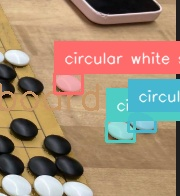
\includegraphics[width=\textwidth]{image1_grounded.jpg}
    \caption{Close-up view with stone segmentation masks and bounding boxes.}
\end{subfigure}
\hfill
\begin{subfigure}[t]{0.48\textwidth}
    \centering
    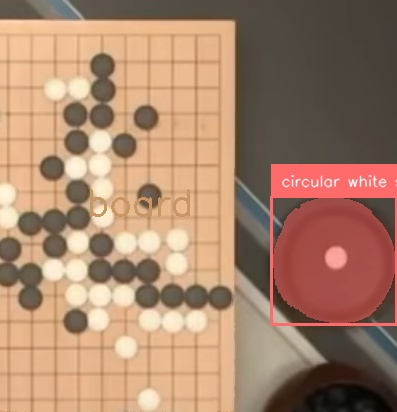
\includegraphics[width=\textwidth]{image3_grounded.jpg}
    \caption{Full board view with board region detection and stone segmentation.}
\end{subfigure}
\caption{Grounded-SAM-2 zero-shot stone detection results. The model detects board regions and individual stones using only natural language prompts, with no task-specific fine-tuning.}
\label{fig:cv}
\end{figure}

%----------------------------------------------------------------------
\section{Robotic Stone Placement}
\label{sec:robot}
%----------------------------------------------------------------------

\subsection{Simulation Environment}

We train a pick-and-place policy in NVIDIA Isaac Lab using a Franka Panda 7-DOF arm with a fixed base and gravity disabled on the robot. The end-effector is a virtual suction cup implemented as distance-based attachment with a 0.1034\,m offset from \texttt{panda\_hand} along $+Z$, chosen over a parallel-jaw gripper because the vertical approach simplifies placement into crowded board regions. The environment runs 2,048 parallel instances on GPU via PhysX at 200\,Hz physics and 50\,Hz control (decimation${}=4$) with $4{\times}$ action repeat, yielding an effective policy rate of 12.5\,Hz. Episodes last 12~seconds (150 policy decisions).

Go stones are modeled as cylinders (diameter 21.9\,mm, height 8.8\,mm, mass 6.8\,g) with analytically computed inertia tensors. The stone spawns at $(0.35, {-}0.15)$ and the target is at $(0.5, 0.15)$ on a table at ground level.

\subsection{Action Representation}

The action space is 8-dimensional: 7~joint position deltas plus 1~binary suction command. Critically, actions are \emph{delta-from-current} joint positions rather than absolute targets:
\begin{equation}
q_{\mathrm{target}} = q_{\mathrm{current}} + a \cdot \delta_{\mathrm{scale}}, \qquad \delta_{\mathrm{scale}} = 0.2\;\mathrm{rad}, \quad a \in [-1, 1]^7.
\end{equation}
By reducing the learning problem to predicting small corrections from the current configuration rather than absolute targets, delta actions avoid compounding integration error and improve training stability.

The actor observation is 39-dimensional: joint positions minus defaults~(7), joint velocities~(7), previous action~(8), end-effector position~(3), stone position~(3), target position~(3), stone-to-tip vector~(3), target-to-stone vector~(3), suction active flag~(1), and attachment flag~(1). The critic receives 3 additional dimensions (stone linear velocity, 42D total).

\subsection{Online IK Teacher and Reward Design}

Rather than behavioral cloning followed by RL fine-tuning---which we found collapses action entropy and causes catastrophic forgetting under PPO---we train PPO from scratch with an online IK teacher providing an auxiliary imitation reward. The teacher is a 7-DOF damped least-squares IK solver with an 8-phase state machine (Reach$\to$Lower$\to$Grasp$\to$Lift$\to$Transport$\to$Place$\to$Release$\to$Retract) that runs in parallel with the student policy across all environments.

The total reward combines a ManiSkill3-style staircase task reward with the imitation signal:
\begin{equation}
r = w_{\mathrm{task}} \cdot r_{\mathrm{task}} + w_{\mathrm{imitate}} \cdot r_{\mathrm{imitate}}, \qquad r_{\mathrm{imitate}} = \frac{1}{d}\sum_{i=1}^{d}\exp\!\bigl({-}5\,(a_i^{\mathrm{s}} - a_i^{\mathrm{t}})^2\bigr).
\end{equation}
The task reward decomposes into sequential stages (Table~\ref{tab:rewards}), where later stages unlock only after earlier ones are satisfied, providing a dense gradient throughout training. Imitation weights are annealed from $w_{\mathrm{imitate}}{=}0.5$ to $0.0$ while task weights grow from $w_{\mathrm{task}}{=}0.5$ to $1.0$ over 300K steps, allowing the policy to bootstrap from teacher guidance then optimize task performance independently.

\begin{table}[t]
\centering
\caption{ManiSkill3-style staircase reward for pick-and-place training. Each stage gates on the previous one being satisfied; the reward range column shows the cumulative contribution.}
\label{tab:rewards}
\small
\begin{tabular}{@{}llc@{}}
\toprule
\textbf{Stage} & \textbf{Condition} & \textbf{Reward range} \\
\midrule
Reach    & EE approaches stone & 0--1 \\
Grasp    & Suction attached     & 0--2 \\
Lift     & Stone raised above table & 0--3 \\
Transport & Stone moved toward target & 0--4 \\
Near target & Stone within proximity & 5--10 \\
Success  & Stone at target + released & 9--20 \\
\bottomrule
\end{tabular}
\end{table}

An adaptive suction curriculum further accelerates learning: the attachment distance threshold starts at 5\,cm and tightens by 30\% whenever fine-accuracy exceeds 15\%, converging to 1\,mm. The policy's binary suction action controls attachment timing, guided by the teacher's imitation signal.

\subsection{Training Configuration}

We train with PPO (clip ratio 0.2, entropy coefficient 0.01, $\gamma{=}0.99$, $\lambda{=}0.95$) using an actor-critic network with hidden layers [256, 128, 64] and ELU activations. The learning rate is $3{\times}10^{-4}$ with adaptive scheduling based on KL divergence, and the initial noise standard deviation is 0.5. No behavioral cloning pretraining is used. Training converges within 2{,}000 iterations (${\sim}$60 minutes wall-clock on an RTX~5070~Ti).

\subsection{Results}

We evaluate three configurations: a pure IK controller baseline, a teacher-assisted residual policy, and a fully standalone learned policy (Table~\ref{tab:placement_results}).

\begin{table}[t]
\centering
\caption{Stone placement accuracy across controller configurations. All use a 1\,mm suction activation threshold.}
\label{tab:placement_results}
\small
\begin{tabular}{@{}lccccc@{}}
\toprule
\textbf{Configuration} & \textbf{Episodes} & \textbf{Median 3D} & \textbf{Mean 3D} & \textbf{$\leq$10\,mm} & \textbf{Success} \\
\midrule
IK baseline (MuJoCo)        & 200     & 3.9\,mm & 3.9\,mm & 100\%  & 100\% \\
Teacher-assisted (residual)  & 5{,}120 & 3.6\,mm & 6.1\,mm & 80.5\% & 100\% \\
Standalone (delta PPO)       & 4{,}096 & 4.2\,mm & 5.8\,mm & 93\%   & 100\% \\
\bottomrule
\end{tabular}
\end{table}

\textbf{IK controller baseline.} A pure damped least-squares IK controller with a 1\,mm suction threshold evaluated in MuJoCo achieves 100\% completion with a constant 3.88\,mm placement error across 200 fixed-position episodes. This represents the physics floor---the systematic offset arising from suction tip geometry during release.

\textbf{Teacher-assisted residual policy.} The IK teacher drives the base trajectory while the RL policy learns additive corrections of $\pm$0.0125\,rad per joint. Over 5,120 evaluation episodes, this achieves 3.6\,mm median 3D error (2.1\,mm mean XY error), with 80.5\% of placements within 10\,mm and 99.7\% within 20\,mm, at 100\% pick-and-place completion. This configuration requires the IK solver at inference time.

\textbf{Standalone learned policy.} The delta-action PPO policy trained from scratch with the online imitation reward achieves 100\% task completion and 93\% fine placement accuracy ($\leq$10\,mm) with a 1\,mm suction threshold, reaching 4.2\,mm median placement error. Crucially, this policy is a fully standalone neural network---no IK solver or teacher is needed at inference. Given that Go board intersections are spaced ${\sim}$22\,mm apart, sub-5\,mm precision is more than sufficient for unambiguous stone placement. The adaptive suction curriculum proved essential: the threshold tightens automatically from 50\,mm to 1\,mm in approximately 1{,}000 iterations as the policy's grasping precision improves, achieving the final accuracy within 2{,}000 total iterations of training.

\subsection{Humanoid Generalization}

To validate the generality of our teacher-student approach, we also implemented the same pipeline for the Unitree G1 humanoid (29-DOF, using the waist and right arm for manipulation). The G1 controller uses the identical ManiSkill3-style staircase reward with an online IK teacher and behavioral cloning warmstart, demonstrating that the approach transfers across substantially different robot morphologies without architectural changes.

%----------------------------------------------------------------------
\section{Discussion and Future Work}
%----------------------------------------------------------------------

\textbf{Integration.} The three components form a complete pipeline: camera image $\to$ stone detection $\to$ board state $\to$ style-aware move prediction $\to$ robotic placement. End-to-end integration and sim-to-real transfer for the manipulation policy remain as future work. We plan to apply domain randomization during simulation training to produce a robust policy that generalizes to real hardware.

\textbf{Era-specific stylistic adaptation.} Our era-specific fine-tuning experiments demonstrate that Go playing styles are temporally distinct and learnable. Models fine-tuned on pre-1900 games gain +7.3\% over the human SL baseline, while 2020s models gain only +1.3\%, reflecting how modern AI-influenced play is already well-represented in the base model. This suggests a two-stage approach for player mimicry: first adapt to the target player's era, then specialize on their individual games. For Nie Weiping, this pipeline achieves 59.4\% top-1 accuracy (+7.7\% over self-play, +4.7\% over humanv0).

\textbf{Manipulation policy.} The standalone PPO policy achieves 4.2\,mm median placement error at 100\% task completion with a 1\,mm suction threshold---well within the 22\,mm grid spacing required for unambiguous Go stone placement. Three key insights drove this result: (i)~delta-from-current actions eliminate the compounding error that plagued absolute action formulations, (ii)~training PPO from scratch with an online imitation reward avoids the catastrophic forgetting of BC-then-RL pipelines, and (iii)~an adaptive suction curriculum that tightens based on measured accuracy accelerates convergence. The key remaining challenge is sim-to-real transfer, where we expect the suction-based end-effector to be more robust than a parallel-jaw gripper given the stones' small, biconvex geometry.

\textbf{Broader impact.} This system could enable accessible Go instruction by physically demonstrating a master player's style, or serve as a research platform for studying human decision-making patterns in strategic games.

%----------------------------------------------------------------------
\section*{Acknowledgements}
%----------------------------------------------------------------------

The robotic pick-and-place simulation environment is adapted from the open-source Isaac Lab project by SamithVa.\footnote{\url{https://github.com/SamithVa/PickAndPlace}}

%----------------------------------------------------------------------
% References
%----------------------------------------------------------------------
\bibliographystyle{plain}
\begin{thebibliography}{10}

\bibitem{silver2016mastering}
D.~Silver, A.~Huang, C.~J. Maddison, et~al.
\newblock Mastering the game of {G}o with deep neural networks and tree search.
\newblock \emph{Nature}, 529(7587):484--489, 2016.

\bibitem{wu2019accelerating}
D.~J. Wu.
\newblock Accelerating self-play learning in {G}o.
\newblock \emph{arXiv preprint arXiv:1902.10565}, 2019.

\bibitem{liu2023grounding}
S.~Liu, Z.~Zeng, T.~Ren, et~al.
\newblock Grounding {DINO}: Marrying {DINO} with grounded pre-training for open-set object detection.
\newblock \emph{arXiv preprint arXiv:2303.05499}, 2023.

\bibitem{ravi2024sam2}
N.~Ravi, V.~Gabeur, Y.-T.~Hu, et~al.
\newblock {SAM}~2: Segment anything in images and videos.
\newblock \emph{arXiv preprint arXiv:2408.00714}, 2024.

\bibitem{schulman2017proximal}
J.~Schulman, F.~Wolski, P.~Dhariwal, A.~Radford, and O.~Klimov.
\newblock Proximal policy optimization algorithms.
\newblock \emph{arXiv preprint arXiv:1707.06347}, 2017.

\end{thebibliography}

%----------------------------------------------------------------------
% NeurIPS Paper Checklist
%----------------------------------------------------------------------
\newpage
\section*{NeurIPS Paper Checklist}

\begin{enumerate}

\item {\bf Claims}
\item[] \textbf{Answer:} Yes. All accuracy numbers are reported with dataset sizes and evaluation methodology.

\item {\bf Limitations}
\item[] \textbf{Answer:} Yes. We discuss the dataset size bottleneck and grasping challenges.

\item {\bf Theory}
\item[] \textbf{Answer:} NA. This is primarily an empirical systems paper.

\item {\bf Experiments}
\item[] \textbf{Answer:} Yes. We report hyperparameters, dataset sizes, model architectures, and training details.

\item {\bf Compute}
\item[] \textbf{Answer:} Yes. All fine-tuning experiments were conducted on a single NVIDIA RTX 5070 Ti GPU.

\item {\bf Code and data}
\item[] \textbf{Answer:} The game records are from public databases. Code will be made available upon publication.

\item {\bf Broader impacts}
\item[] \textbf{Answer:} Yes. Discussed in Section~5.

\end{enumerate}

%----------------------------------------------------------------------
\section*{LLM Disclosure}
%----------------------------------------------------------------------

Large language models (Claude, Anthropic) were used as coding assistants throughout this project for tasks including data pipeline development, experiment orchestration, hyperparameter search, and manuscript drafting. All experimental results were independently verified, and the authors take full responsibility for the correctness of the reported findings.

%----------------------------------------------------------------------
\section*{Target Venue}
%----------------------------------------------------------------------

This work is targeted at the ICRA 2026 Workshop: \textit{Bridging the Gap between Robot Learning and Human-Robot Interaction}.

\end{document}
